\documentclass[a4paper,12pt]{extarticle}
\usepackage{geometry}
\usepackage[T1]{fontenc}
\usepackage[utf8]{inputenc}
\usepackage[english]{babel}
\usepackage{amsmath}
\usepackage{amsthm}
\usepackage{amssymb}
\usepackage{fancyhdr}
\usepackage{setspace}
\usepackage{graphicx}
\usepackage{colortbl}
\usepackage{tikz}
\usepackage{pgf}
\usepackage{subcaption}
\usepackage{listings}
\usepackage{indentfirst}
\usepackage[colorlinks,citecolor=blue,linkcolor=blue,bookmarks=false,hypertexnames=true, urlcolor=blue]{hyperref} 
\usepackage[noabbrev]{cleveref}
\usepackage{indentfirst}
\usepackage{mathtools}
\usepackage{booktabs}
\usepackage[flushleft]{threeparttable}
\usepackage{tablefootnote}
% \usepackage{refcheck}

\usepackage{chngcntr} % нумерация графиков и таблиц по секциям
\counterwithin{table}{section}
\counterwithin{figure}{section}
\DeclareMathOperator*{\argmin}{arg\,min} 
\graphicspath{{graphics/}}%путь к рисункам

\makeatletter
\renewcommand{\@biblabel}[1]{#1.} % Заменяем библиографию с квадратных скобок на точку:
\makeatother

\geometry{left=2.5cm}% левое поле
\geometry{right=1.5cm}% правое поле
\geometry{top=1.5cm}% верхнее поле
\geometry{bottom=1.5cm}% нижнее поле
\renewcommand{\baselinestretch}{1.25} % междустрочный интервал
\RequirePackage{float}                

\renewcommand{\theenumi}{\arabic{enumi}.}% Меняем везде перечисления на цифра.цифра
\renewcommand{\labelenumi}{\arabic{enumi}.}% Меняем везде перечисления на цифра.цифра
\renewcommand{\theenumii}{\arabic{enumii}.}% Меняем везде перечисления на цифра.цифра
\renewcommand{\labelenumii}{\arabic{enumi}.\arabic{enumii}.}% Меняем везде перечисления на цифра.цифра
\renewcommand{\theenumiii}{\arabic{enumiii}.}% Меняем везде перечисления на цифра.цифра
\renewcommand{\labelenumiii}{\arabic{enumi}.\arabic{enumii}.\arabic{enumiii}.}% Меняем везде перечисления на цифра.цифра

% \crefname{section}{глава}{глава }
% \Crefname{section}{Глава}{Глава }
% \crefname{figure}{рис.}{рис. }
% \Crefname{figure}{Рис.}{Рис. }
% \crefname{table}{табл.}{табл. }
% \Crefname{table}{Табл.}{Табл. }

\begin{document}

\section{Introduction to the problem}

Orienteering is a sport that requires athletes to run with a map, following certain cet of rules about the destination of the run.
In most cases, they shall get to specified locations in specified order as fast as possible.
Orienteering can be done in cities, forests, mountains, malls, and so on.

The only thing that athlete has after the race is the map, and for professional athletes it is crucial to do post-analysis of their race performance.
For some races, such as city races, route choice problem is crucial.
And it is important to find all routes available and compare their length.

\subsection{Problem statement}

This project aims to create a tool that will do analysis of routes for orienteering city races.
Our tool allows to find the optimal route for each control of an orienteering course, but we also propose a theoretical
algorithm to find multiple different optimal paths as well.

\subsection{Related applications and technologies}

\begin{enumerate}
    \item Strava is a social network for runners that allows uploading your own gps routes and put a map underneath them.
While it is helpful, it does not solve the route problem, it only helps with visualisation.
    \item Livelox is a website created for orienteering competitions, where jury can upload map with distance configuration, and athletes can upload their GPS tracks.
The data used by organisers is private. 
    \item The maps and courses are usually created with specific software such as OCAD and openorienteering. 
Such software creates data files that have precise vectorized description of a map, but these files are mostly private, and community only has a jpeg version of a map.
    \item Tools, similar to our project, are used for world cup translations, but they are propriate and use private data as well.
\end{enumerate}

\section{Implemented methods}

We created a pipeline consisting of several algorithms that decomposed the problem and provided step by step solution with the ability to change the implementation of any block in case results are not good enough.
Because of the fact that one stage might heavily depend on previous one, we decided that it is necessary to allow manual modification of intermediate data, because otherwise we will stack the error.

Overall, the developed pipeline is the following:
\begin{enumerate}
\item Extraction of course layer with CNN model
\item Extraction of obstacles with U-Net
\item Detection of circles with hough circles modification and kernel scoring
\item Detection of triangles based on OpenCV polygon detection
\item Extraction of information about the course configuration with TSP solver on course layer with special scoring matrix
\item Selection of the best routes for each control with $A^*$ algorithm.
\end{enumerate}


\subsection{Semantic segmentation for layers separation}

There are no labelled public datasets of orienteering city maps, so we found some open archives of orienteering maps and selected a sample of 50 maps by hand.
To label this data for semantic segmentation problem, we used a special python package labelme, that allows to manually select shapes on top of the image given.
We labelled 27 images for segmentation of runnable layers and 12 full courses.

Labelme produces json array with description of all the shapes (we used lines, circles, and polygons).
To create a mask out of the json description of a shape border, following algorithm was used:
\begin{enumerate}
    \item Take shapes one by one and determine its bounding box
    \item For every pixel in bounding box, check if pixel belongs to a shape
    \item To finding if the point is inside the shape, point-to-segment distance was used for lines, circle equation was used for circles and common algorithm for polygons that shoots the ray from the point and calculates number of intersections with edges.
\end{enumerate}


\subsubsection{Detection of course layer}

To try and outperform the naive implementation, we developed and trained a CNN to detect the unrunable layers, e.g the layers that notated where the start/end points of a track lied, the connections between tracks, and the labels for each track.
The motivation for creating this CNN was that we could not be sure that a naive implementation of removing layers based on color alone would work well, and we hoped that a simple CNN could detect connected circles, triangles, and lines of the same color and thickness in order to remove them from the final map. 

In order to train the CNN with a limited dataset, we took maps without extra layers, in other words maps that were ready for path detection, and added layers on top of them so that we could have ample training and validation sets.
This included drawing a random number of circles, lines, and text using cv2 functions, ensuring that the locations of the circles were spread out and the lines connected the circles, and using a variety of colors (though uniform per training image).
All in all it was fairly simple and allowed us to produce however many training/validation images as we wanted.

To produce the masks for the training and validation sets, all that needed to be done was feed in the color that was used to create the figures on the training/validation images into a function that took a “bitwise and” of the image and a mask of that color.
Then just converting the mask to black and white produced good results.

We created a simple CNN model with 2 convolution layers and no pooling layers, figuring that all the CNN would really do is learn the intended colors to remove, since the figures to be removed were uniformly colored.
The model would take in a colored 200x200 random segment of each colored image, and output a black/white mask as intended.
For the model we experimented with different loss functions, and decided on Binary Cross Entropy loss, which is used commonly for binary classification tasks.
For the optimizer, we learned that the Adam optimizer produced results similar to though more effective than Stochastic Gradient Descent, and ran with that.

Eventually we realized that for the task of circle detection we needed the model to do more than just separate the layers based on color.
There were often parts of the map that were the same color as the layers we intended to remove, and we didn't want to segment them in the layer detection model.
This was because the circle detection was much less effective if there were layers interrupting the circles.
So we attempted to reconfigure the model to ideally just identify the circles and lines, ignoring other figures like labels of the circles and other figures in the map (areas that were out of bounds often were colored the same as the circles/lines).
Our reasoning for the current state of the model was that it should have already been able to do more than simple color identification, if we just modified the training masks to only include the lines and circles.
We did this and also attempted to incorporate max pooling which should have made line detection easier.
Unfortunately this model did not produce good results, and we were ultimately unable to use it.

Using the images and masks that we had created, we made tensors which could be fed into pyTorch data loaders.
This involved creating random crops of the masks and images.
One problem we had to overcome, which turned out to be relatively simple, was ensuring that the random crops were of the same section for the images and corresponding masks.
With our training and validation data loaders, we were able to train the model in the corresponding fashion.

Our number of epochs was higher than we would have liked, but we did get our average validation below 0.5 so we were fine with waiting for the model to finish training.

With our model fully trained, we were able to test it on a testing set that was filled with maps with layers on top.
While it did produce great results on maps where the layers to be removed were the only ones of that color, since the model was essentially just detecting the colors of the layers it produced a decent amount of noise on non-ideal maps.
Before attempting to modify the model to only separate circles/lines, we thought that we would be able to remove the noise in order to isolate the intended figures for the later circle detection algorithm.
However, as we discovered the main problem wasn’t removing noise, which did not really hinder the way we detected the circles, but rather the presence of larger figures like pink areas on the map or the numerical labels of the circles. 

\subsubsection{Detection of runnable layer}

For detection of a runnable layer, we tried CNN model and U-Net model.
Advantage of the U-Net is its ability to always have a context of real pixel values.

\subsection{Detection of course configuration}

Course configuration consists of triangle, which is a start, circles, that represent controls, and lines that are used for connection.
In general, there are many possibilities for race rules, that may result in map having several start points, more than two connections for a control or even no connections at all.
We decomposed our detection process the way that shapes detection is separated from connecting objects so intermediate data might still be useful.
Consiedring connections between controls, there might be many issues, but for the sake of simplicity, we limited out problem to courses when  configuration is a permutation of circles, which is the most common one.

\subsubsection{Algorithm for triangle detecction}

To find a start is a problem of finding a triangle. We know that the triangle is equilateral. To find it, we need to address the challenge of a noise in the data. In general, openCV provides a way to find a custom polygon. The problem with the method is that it expects polygon to be filled, when triangle from our dataset only has contours. Not only the triangle has contours, but it also has adjacent line, so using default algorithm is not an option.
Our pipeline uses dilation to expand triangle borders until it becomes solid, so the contour is closed. Then using erosion it is possible to remove external pixels both for triangle and for lines around them -- the only difference is lines disappear completely and triangle has internal solid part left. This part can be detected with default openCV tools 

[DEMO PICTURE]

The issue we found with the algorithm is that it is dependent on two thresholds: dilation and erosion parameters. ideally, D - E = W, where W is a line width in pixels, and D is third to half of triangle size.


\subsubsection{Algorithm for circle detection}

To find circles, Hough circles method was used as the first approach. the problem with this method is that it detects all circles, not only fixed radius. 

[DEMO WITH A PROBLEM PICTURE]

Also circles are corrupted and they have adjacent lines as well. So we came up with a scoring system that estimates if region has circle or not.

Our algorithm selects interesting regions and then checks if region is circle or not. Regions are squares that expect circles of fixed radius. We consider every region that has more than A pixels interesting.

To check the region, we apply a kernel that favors regions with pixels on the border and penalties pixels inside of the circle.

[DEMO PICTURE]

Our algorithm has 3 prerequired parameters: radius, score for selection of interesting areas and threshold for getting a circle.


\subsubsection{Algorithm for configuration detection}

Because we know that configuration is a permutation. all we have to do is to find a permutation of points (control points + start), where each pair of adjacent points is connected in the course layer.
Lines can intesectm, they can miss some part, they might not me straight, so there is no way to find the exact permutation.

So, to find a permutation, we construct a pairwise scoring, which shows how close the points are.
Then we solve TSP problem with annealing-based TSP-solver.

Scoring takes two things into account:
\begin{enumerate}
    \item Most of the connections are straight lines.
    \item Some connections are not.
\end{enumerate}

We found out that it is helpful to create two scores.
First srore tries to find straight lines and is based on number of course layer pixels on the straight line, that weren't set.

Second score tries to find any possible way to connect two points and estimates, how long this connection line would be.
The algorithm to find such score is quite complicated: it creates quadtree for an course layer, and then creates a graph from adjacent vertices of quadtree.
On the graph vertices it is possible to run $A^*$, and it is the way to compress graph.
Running $A^*$, we not only allow connecting pixels from couse layer, but also adding pixels that were not set, with a penalty.

\subsection{Shortest path analysis}

We applied $A^*$ to the obstable layer to find optimal pathes.

\section{Result: a Streamlit-based web application}

There are many steps of the pipeline where something can go wrong, so as we are doing proof-of-concept, we made a web application that allowed us to modify thresholds interactively and correct output of detectors if they are wrong. it is used instead of web components that could be done by cool web developer.

Application was built on top of Streamlit framework which allows to use Python for creating simple interactive websites. Streamlit allows caching results and tune thresholds easily (not as easy as with real widgets but it is still manageable).


\section{Extra: ideas for the future}

The problem that is important for the application is it’s ability to show several best ways that aren’t the same in terms of “how route goes around obstacles”. We managed to understand a problem and think of a way to solve it, but it is a challenging task that would require twice as much time as everything else.
Two routes are equivalent if they can be continuously modified so one turns into another without crossing the obstacles.
To address this problem, it is possible to build Voronoi diagram-like structure, separating each pixel based on the closest obstacle. It would mean that every pixel is now between two obstacles and each path can be classified by sequence of regions. then it is possible to compress each region into a single vertex and find several shortest paths on a new graph. But this is a really challenging task for future work.


\newpage
\appendix
\section{Appendix}
\subsection{Figures}


\begin{figure}[H]
    \centering
    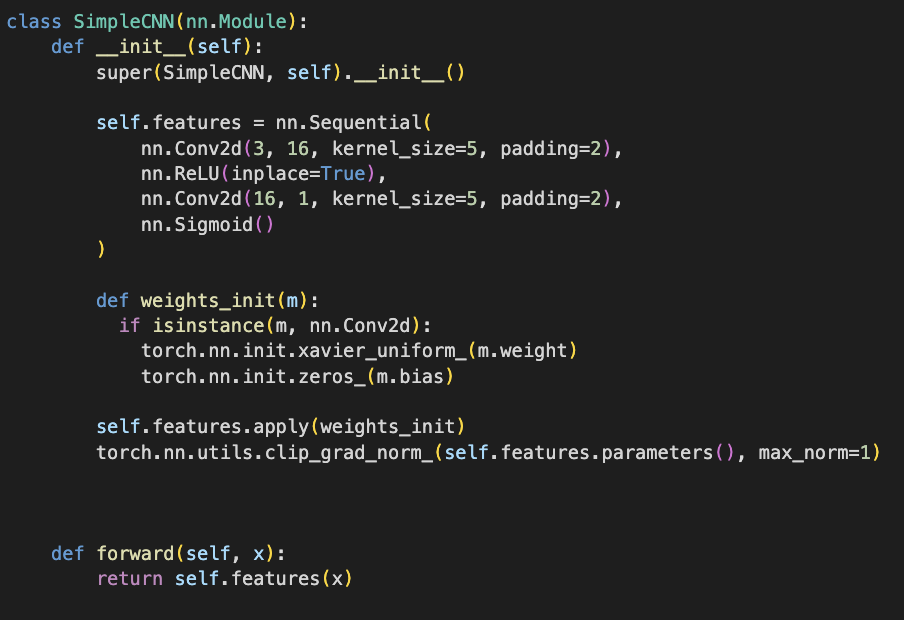
\includegraphics[width=\linewidth]{CNN simple model.png}
    \captionof{figure}{Simple CNN Model}
    \label{fig:simple-CNN}
\end{figure}

\begin{figure}[H]
    \centering
    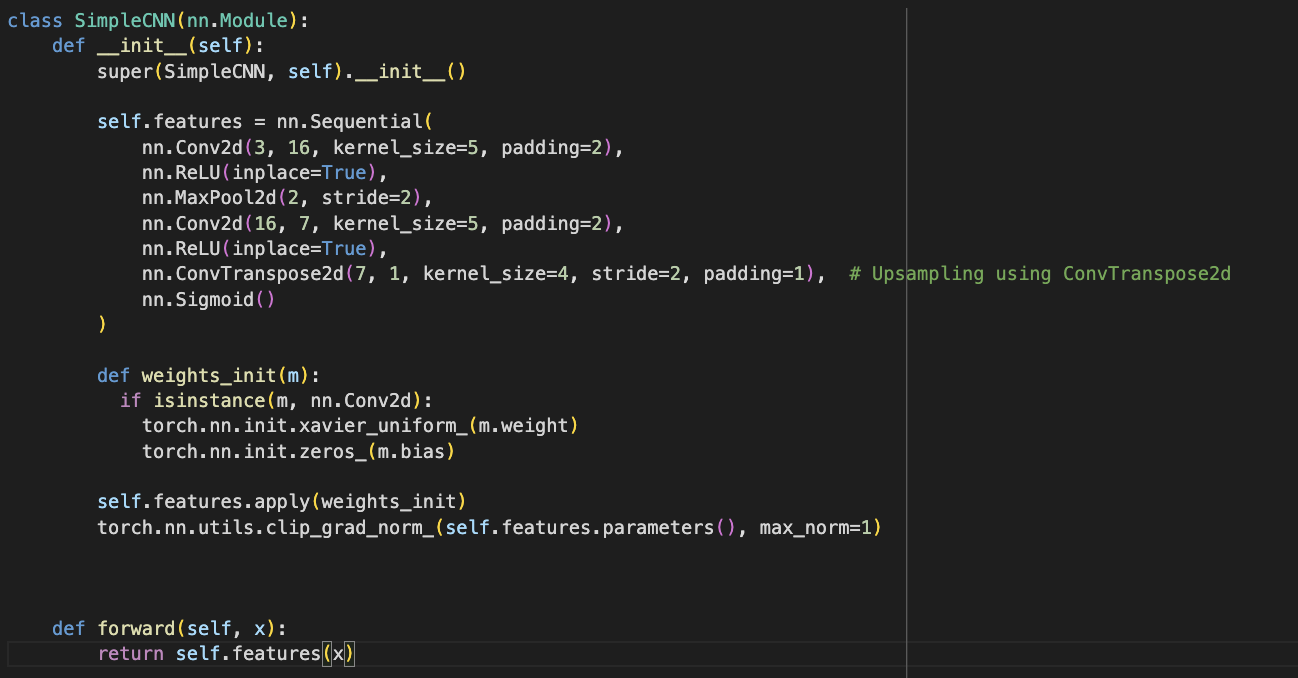
\includegraphics[width=\linewidth]{CNN model pooling.png}
    \captionof{figure}{CNN Model with Pooling}
    \label{fig:pooling-CNN}
\end{figure}

\begin{figure}[H]
    \centering
    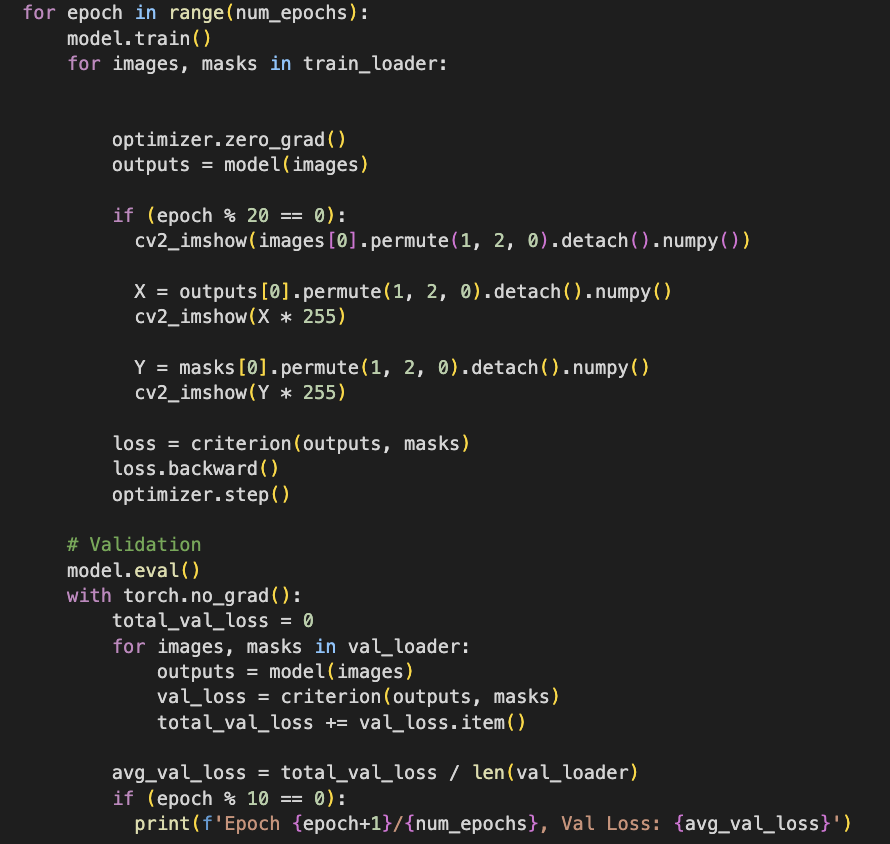
\includegraphics[width=\linewidth]{CNN training loop.png}
    \captionof{figure}{Model Training Loop}
    \label{fig:training-loop}
\end{figure}

\begin{figure}[H]
    \centering
    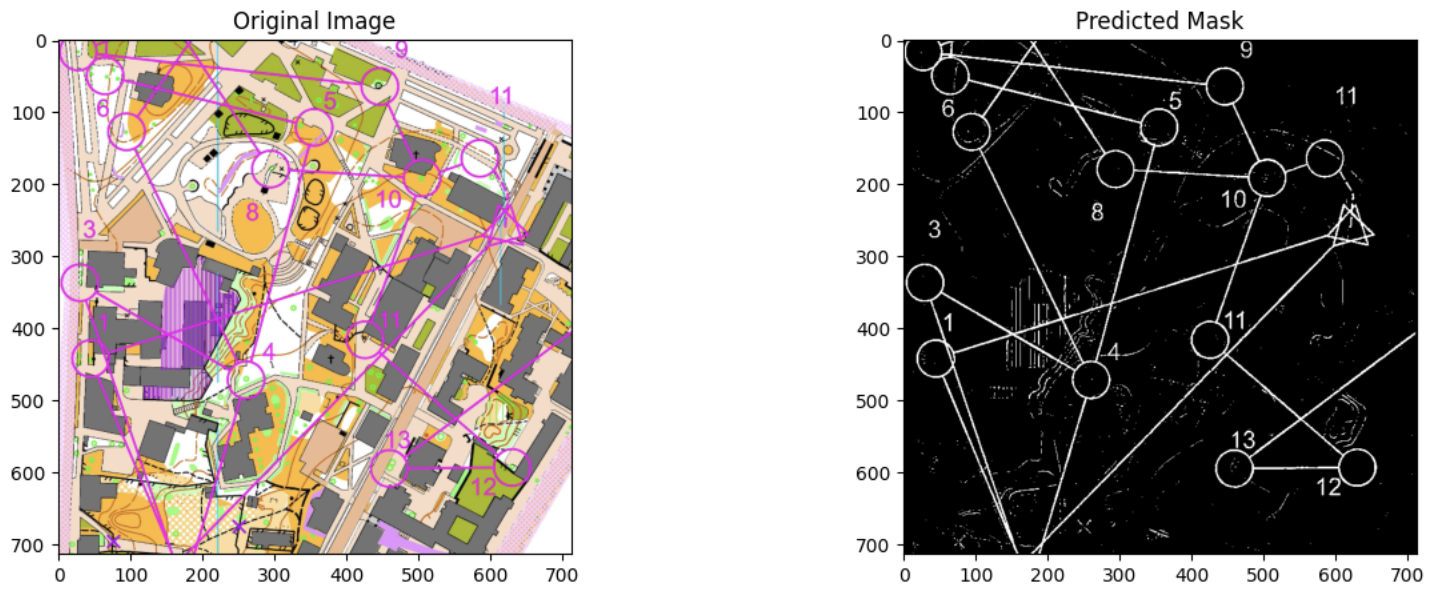
\includegraphics[width=\linewidth]{Predicted mask.png}
    \captionof{figure}{Predicted Mask from Image}
    \label{fig:predicted-mask}
\end{figure}
  

\newpage

% \nocite{*}


\begin{thebibliography}{00}
\bibitem{b12} DSLab, --- URL: 
\bibitem{b12} OpenCV, --- URL: 
\bibitem{b12} U-Net, --- URL: 
\bibitem{b12} Streamlit, --- URL: 
\bibitem{b12} Strava, --- URL: 
\bibitem{b12} Livelox, --- URL: 
\bibitem{b12} World cup live translation, --- URL: 
\bibitem{b12} hough circles, --- URL: 
\bibitem{b12} check that point is into triangle, --- URL: 
\bibitem{b12} A star on quadtree, --- URL: 
\bibitem{b12} voronoi on polygons, --- URL: 
\bibitem{b12} pytorch and keras, --- URL: 
\bibitem{b12} augmentation, --- URL: 
\bibitem{b12} semantic segmentation --- URL: 
\bibitem{b12} labelme --- URL: 
\bibitem{b12} jaccard metric --- URL: 

\end{thebibliography}
	
	
\end{document}
